% IEEE conference version (6 pages or less).
% Built on the official IEEE conference LaTeX template (version 6/27/2024,
% IEEEtran.cls V1.8b) from https://www.ieee.org/conferences/publishing/templates.
% Do not change margins, fonts, or column settings.
%
% Status: study design. No solver, PINN, or energy run exists yet.
% Sources of truth: docs/research-plan.md, docs/problem-definition.md,
% docs/model-equations.md, docs/reference-solution.md,
% docs/training-pipeline.md, docs/gap-analysis.md, docs/gap-evidence.md.
\documentclass[conference]{IEEEtran}

\usepackage{cite}
\usepackage{amsmath,amssymb,amsfonts}
\usepackage{graphicx}
\usepackage{textcomp}
\usepackage{xcolor}
\usepackage{booktabs}
\usepackage{tikz}
\usetikzlibrary{positioning,arrows.meta,fit,calc}
\usepackage[hidelinks]{hyperref}
\graphicspath{{../shared/figures/}}

\newcommand{\Nstar}{N^{\ast}}

\begin{document}
\bstctlcite{IEEEexample:BSTcontrol}

\title{Reaching the Energy and Computational Break-Even Point Between PINNs, and Classical Solvers}

\author{\IEEEauthorblockN{Anonymous Author(s)}
\IEEEauthorblockA{\textit{Affiliation withheld for review}}
}

\maketitle

\begin{abstract}
A parametric physics-informed neural network (PINN) is trained once for a whole family of problems. After that, each new parameter setting needs only one forward pass. Training, however, spends energy before the first answer. We ask how many new queries it takes before the PINN's total electricity falls to that of a finite-difference solver at the same accuracy. We ask the same question for runtime. Published comparisons of PINNs with classical solvers report time for single solves. In our search, none measures electricity across a parameter family. This paper presents a study design for that measurement. It reports no measured results. The workload is steady diffusion on the unit square, where two parameters set the conductivity. Both methods answer the same unseen parameters on one output grid, at relative L2 errors of 1\% and 0.1\%. The design has four parts: a cost model that charges failed training runs, an accuracy check that both methods must pass, a counter-based energy protocol on one machine, and a rule that sorts each result into one of four outcomes. A crossover that is absent or very far away is a valid result.
\end{abstract}

\begin{IEEEkeywords}
physics-informed neural networks, energy measurement, green computing, finite differences, break-even analysis
\end{IEEEkeywords}

% ===========================================================================
\section{Introduction}

Physics-informed neural networks (PINNs) learn the solution of a partial differential equation (PDE) by penalizing the equation's residual~\cite{raissi2019,karniadakis2021,cuomo2022,toscano2025}. A parametric PINN also takes the PDE parameters as inputs. One trained network then covers a whole family of problems~\cite{sun2020,wang2021deeponet}. A new parameter setting costs one forward pass. A classical solver must solve a new linear system each time. Training, however, costs energy before the first answer. Work on green computing asks that such costs be measured and reported~\cite{strubell2019,schwartz2020,patterson2022}. This leads to a simple question. How many new queries does it take before the PINN's training energy is paid back?

In the search recorded for this project, we found no published work that answers it. Studies that compare PINNs with classical solvers time one problem at a time~\cite{grossmann2024,chuang2022,markidis2021}. In nearly every test, the classical solver was faster at equal or better accuracy~\cite{grossmann2024}. In these papers, PINN training took from about 69 times~\cite{markidis2021} to more than 28\,000 times~\cite{chuang2022} as long as one classical solve. We computed these ratios from the reported times. They come from PINNs trained for one problem, often on other hardware than the classical solver, so they do not predict our case. Work on many queries studies supervised neural operators instead. One preprint reports that no Fourier neural operator with error below 1\% broke even before 31\,000 queries~\cite{huang2026review}. Another defines break-even for neural solvers in wall-clock time~\cite{zhang2026}. None of these studies reports energy in joules. The closest energy studies estimate carbon with software tools~\cite{kapoor2025} or meter neural inference only~\cite{yoo2026}.

Simple proxies for energy can mislead. Across model architectures, operation counts explained little of the variation in energy ($R^2=0.083$)~\cite{henderson2020}. In a PDE forecasting preprint, runtime alone was an unreliable proxy for carbon cost~\cite{wilson2025}. A faster method may still use more energy. So we measure the energy and runtime break-even points separately.

A fair measurement has to handle three problems. First, both methods must reach the same accuracy, and the classical solver must be efficient. McGreivy and Hakim found that 79\% of the reviewed papers that claimed to beat a standard numerical method used a weak baseline~\cite{mcgreivy2024}. Second, the methods may run on different devices. Grossmann et~al. ran the PINN on a GPU and the classical solver on CPU cores~\cite{grossmann2024}. Chuang and Barba used different machines~\cite{chuang2022}. Energy must then be read inside one declared boundary. Third, PINN training can stall or fail~\cite{krishnapriyan2021,wang2022ntk,rathore2024}. Failed runs also use energy.

This paper sets out a study design that handles these problems for one workload: 2D steady diffusion with two conductivity parameters, on one machine. It reports no measured results. Our contributions are:
\begin{itemize}
\item a break-even cost model for energy and runtime that charges failed training runs and the cost of checking accuracy, with a rule that sorts each result into one of four outcomes (Section~\ref{sec:model});
\item a design for a matched-accuracy comparison, with an accuracy gate on unseen parameters, a finite-difference solver that keeps all valid reuse, and a parametric PINN with exact boundary values (Sections~\ref{sec:setup} and~\ref{sec:solvers});
\item a measurement protocol that reads both methods inside one energy boundary, keeps setup, training, and query costs apart, and logs every run (Section~\ref{sec:measure}).
\end{itemize}
Fig.~\ref{fig:pipeline} shows how these parts fit together.

\begin{figure*}[t]
\centering
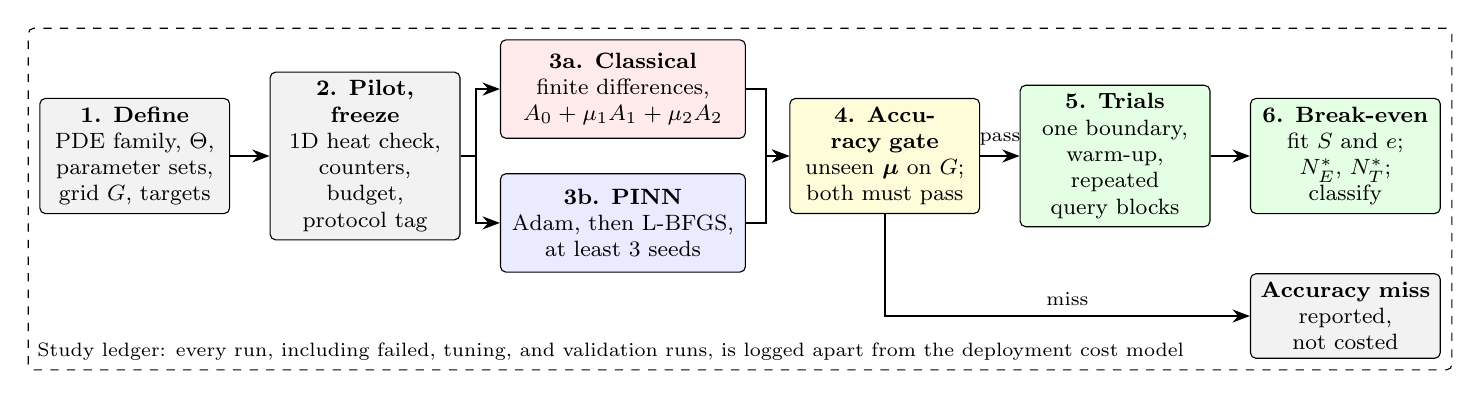
\begin{tikzpicture}[
  font=\footnotesize,
  >={Stealth[length=2.2mm]},
  box/.style={draw, rounded corners=2pt, align=center, text width=2.2cm, minimum height=1.25cm, inner sep=3pt, fill=#1},
  box/.default=white,
  arr/.style={->, thick},
  node distance=0.5cm
]
\node[box=gray!10] (def) at (0,0) {\textbf{1. Define}\\ PDE family, $\Theta$,\\ parameter sets,\\ grid $G$, targets};
\node[box=gray!10, right=of def] (pilot) {\textbf{2. Pilot, freeze}\\ 1D heat check,\\ counters, budget,\\ protocol tag};
\node[box=red!8, right=of pilot, yshift=0.85cm, text width=2.9cm] (fd) {\textbf{3a. Classical}\\ finite differences,\\ $A_0+\mu_1A_1+\mu_2A_2$};
\node[box=blue!8, right=of pilot, yshift=-0.85cm, text width=2.9cm] (pinn) {\textbf{3b. PINN}\\ Adam, then L-BFGS,\\ at least 3 seeds};
\node[box=yellow!15, anchor=west] (gate) at ($(fd.east)!0.5!(pinn.east)+(0.55,0)$) {\textbf{4. Accuracy gate}\\ unseen $\boldsymbol{\mu}$ on $G$;\\ both must pass};
\node[box=green!10, right=of gate] (trial) {\textbf{5. Trials}\\ one boundary,\\ warm-up, repeated\\ query blocks};
\node[box=green!10, right=of trial] (be) {\textbf{6. Break-even}\\ fit $S$ and $e$;\\ $\Nstar_E$, $\Nstar_T$;\\ classify};
\node[box=gray!10, below=0.75cm of be, minimum height=0.8cm] (fail) {\textbf{Accuracy miss}\\ reported, not costed};
\draw[arr] (def) -- (pilot);
\draw[arr] (pilot.east) -- ++(0.2,0) |- (fd.west);
\draw[arr] (pilot.east) -- ++(0.2,0) |- (pinn.west);
\draw[arr] (fd.east) -- ++(0.25,0) |- (gate.west);
\draw[arr] (pinn.east) -- ++(0.25,0) |- (gate.west);
\draw[arr] (gate) -- node[above, font=\scriptsize]{pass} (trial);
\draw[arr] (trial) -- (be);
\draw[arr] (gate.south) |- node[pos=0.75, above, font=\scriptsize]{miss} (fail.west);
\node[draw, dashed, rounded corners=2pt, fit=(def)(fd)(pinn)(be)(fail), inner sep=4pt, label={[font=\scriptsize, anchor=south west]south west:Study ledger: every run, including failed, tuning, and validation runs, is logged apart from the deployment cost model}] {};
\end{tikzpicture}
\caption{Study pipeline. The pilot ends in a frozen protocol. The two solvers are then built in parallel and meet at one accuracy gate on unseen parameters. Only targets that both methods pass go on to the energy and runtime trials.}
\label{fig:pipeline}
\end{figure*}

% ===========================================================================
\section{Related Work}\label{sec:related}

\subsection{PINNs Against Classical Solvers}
Table~\ref{tab:related} summarizes the closest studies. Three studies compare a PINN with a classical solver on single problems, and all three measure time~\cite{grossmann2024,chuang2022,markidis2021}. Physics-informed DeepONets were up to three orders of magnitude faster than a conventional solver per query. That speedup is for inference with a trained model and leaves out training~\cite{wang2021deeponet}. Two preprints give break-even counts, but for supervised neural operators~\cite{huang2026review,zhang2026}. Kapoor et~al. model the carbon of neural PDE solvers over many inferences, with no classical solver to compare against~\cite{kapoor2025}. No row measures energy with hardware counters.

\begin{table}[t]
\caption{Closest studies and what they measure}
\label{tab:related}
\centering
\footnotesize
\setlength{\tabcolsep}{2.5pt}
\begin{tabular}{@{}lllll@{}}
\toprule
Study & Model & Classical rival & Many queries & Cost \\
\midrule
Grossmann~\cite{grossmann2024} & PINN & FEM & No & Time \\
Chuang~\cite{chuang2022} & PINN & Finite diff. & No & Time \\
Markidis~\cite{markidis2021} & PINN & PETSc CG & No & Time \\
Wang~\cite{wang2021deeponet} & PI-DeepONet & Spectral & Yes & Query time \\
Huang~\cite{huang2026review}$^{\mathrm{a}}$ & FNO & FV, AMG-CG & Yes & Solves, time \\
Zhang~\cite{zhang2026}$^{\mathrm{a}}$ & Operators & Coarse num. & Yes & Time \\
Kapoor~\cite{kapoor2025}$^{\mathrm{a}}$ & PINN, ops. & None & Yes & Est. carbon \\
This design & PINN & Finite diff. & Yes & Time, joules \\
\bottomrule
\multicolumn{5}{@{}l}{$^{\mathrm{a}}$Preprint. Rows follow the project's evidence matrix.}
\end{tabular}
\end{table}

\subsection{Training a PINN}
PINN training is hard, and its cost varies. PINNs can fail to learn convection, reaction, and diffusion problems~\cite{krishnapriyan2021}. Loss terms can compete~\cite{wang2021gradient}, and they can train at different rates~\cite{wang2022ntk}. The loss is ill conditioned, and Adam followed by L-BFGS beat either optimizer alone~\cite{rathore2024}. In 32-bit floats, PyTorch L-BFGS can stop early on rounding noise~\cite{xu2025}. Better optimizers can raise accuracy, and small networks can then be enough~\cite{urban2025,wang2025soap}. These findings set our training design.

\subsection{Measuring Energy}
Henderson et~al. proposed reporting energy from hardware counters~\cite{henderson2020}. Intel RAPL readings for the CPU and memory are highly correlated with plug power~\cite{khan2018}. The NVIDIA built-in sensor samples only part of the runtime on some recent GPUs~\cite{yang2024}. Software power meters differ from physical meters~\cite{jay2023,bouza2023}. In one benchmark, changing settings alone sometimes cut inference energy by more than 40\%~\cite{chung2025}. MLPerf Power gives rules for repeatable power tests~\cite{mlperfpower2025}.

% ===========================================================================
\section{Problem Setup}\label{sec:setup}

\subsection{Diffusion Family}
The main problem is steady diffusion on $\Omega=(0,1)^2$:
\begin{equation}
-\nabla\cdot\bigl(k(\mathbf{x};\boldsymbol{\mu})\,\nabla u\bigr)=f \ \text{in}\ \Omega, \qquad u=0 \ \text{on}\ \partial\Omega.
\label{eq:pde}
\end{equation}
Two parameters $\boldsymbol{\mu}=(\mu_1,\mu_2)\in\Theta$ enter only through the conductivity $k$. The working candidate is
\begin{equation}
k=1+\mu_1x+\mu_2y,\qquad \Theta=\left[-\tfrac14,\tfrac14\right]^2,\qquad f=1.
\label{eq:k}
\end{equation}
This gives $\tfrac12\le k\le\tfrac32$, so every query is well posed. The pilot confirms or replaces this candidate. Geometry, source, and boundary values stay fixed. A 1D heat problem with a known solution is used first, as a pilot.

\subsection{Queries}
A query gives one unseen parameter pair $\boldsymbol{\mu}^\ast$. The answer is $u$ at the $M$ points of a fixed output grid $G$. The whole field counts as one query. The query cost covers all the work needed for that answer. For the classical solver, this is forming the matrix, solving, and mapping to $G$. For the PINN, it is one batched forward pass over $G$, with the data moved to and from the device. Both methods answer the same unseen parameters in the same order. No identical query is repeated, so caching gives no advantage.

\subsection{Accuracy Gate}
On $G$, the error of an answer $\hat u$ is
\begin{equation}
\varepsilon(\boldsymbol{\mu})=\lVert\hat u-u_{\mathrm{ref}}\rVert_2\,/\,\lVert u_{\mathrm{ref}}\rVert_2 .
\label{eq:err}
\end{equation}
The targets are $10^{-2}$ and $10^{-3}$, with $10^{-4}$ optional. The reference comes from finer grids with a Richardson check. A method passes a target only on unseen parameters, and the corners of $\Theta$ are included. The team still has to choose between the worst case and a stated quantile. The same rule applies to both methods. Energy trials for a target start only when both methods pass it. A miss is reported as a result and kept out of the cost comparison.

% ===========================================================================
\section{Break-Even Model}\label{sec:model}

\subsection{Cumulative Cost}
For one target and one machine, the energy after $N$ queries is
\begin{equation}
E_P(N)=S_P+N e_P,\qquad E_C(N)=S_C+N e_C .
\label{eq:cost}
\end{equation}
Here $S$ is the setup energy, $e$ is the mean energy per query, and $P$ and $C$ mark the PINN and the classical solver. The two lines meet at
\begin{equation}
\Nstar_E=\frac{S_P-S_C}{e_C-e_P}.
\label{eq:nstar}
\end{equation}
The runtime crossover $\Nstar_T$ uses times in place of energies. If $S_P>S_C$, the PINN catches up only when $e_P<e_C$. The two crossovers need not match.

\subsection{What Setup Includes}
Setup must include the cost of failure. Let $\bar E_{\mathrm{train}}$ be the mean energy of one training attempt and $q$ the share of attempts that pass the gate. If the policy is to retrain until an attempt passes, the expected number of attempts is $1/q$, so
\begin{equation}
S_P=S_{\mathrm{prep}}+S_{\mathrm{val}}+\bar E_{\mathrm{train}}/q .
\label{eq:retry}
\end{equation}
$S_{\mathrm{prep}}$ is model setup. $S_{\mathrm{val}}$ covers the reference solves for validation and the monitoring during training. The policy also caps the number of attempts. If none passes, the PINN fails that target. The classical side is treated the same way: $S_C$ includes the grid study that picked the grid. We report each crossover with and without these accuracy-checking terms. Tuning energy is reported as a separate variant. Table~\ref{tab:terms} lists every term.

\begin{table}[t]
\caption{What each cost term includes}
\label{tab:terms}
\centering
\footnotesize
\setlength{\tabcolsep}{3pt}
\begin{tabular}{@{}lp{6.4cm}@{}}
\toprule
Term & Contents \\
\midrule
$S_C$ & Grid, sparsity pattern, $A_0,A_1,A_2$, output map, grid study \\
$e_C$ & Form $A(\boldsymbol{\mu}^\ast)$, solve, map to $G$ \\
$S_P$ & Setup, validation solves, monitoring, training divided by $q$ \\
$e_P$ & Fill $\boldsymbol{\mu}^\ast$, forward pass on $G$, return output \\
Variant & $S_P$ plus tuning energy \\
Ledger & Every run: pilot, tuning, failures, repeats \\
\bottomrule
\end{tabular}
\end{table}

\subsection{Four Outcomes}
Let $\Delta S=S_P-S_C$ and $\Delta e=e_C-e_P$, and let $N_{\max}$ be the largest query count measured. We use 95\% intervals from Section~\ref{sec:measure}. If the interval of $\Delta e$ contains zero, the slopes cannot be told apart, and the result is an uncertain crossing. Otherwise let $I$ be the interval of $\Nstar$. Fig.~\ref{fig:outcomes} sketches the four classes:
\begin{enumerate}
\item \emph{Crossing in measured range}: $I\subset(0,N_{\max}]$.
\item \emph{One method cheaper throughout}: $I$ lies at or below zero. Then $\Delta S$ and $\Delta e$ have opposite signs, and the lines do not cross for $N\ge0$.
\item \emph{Uncertain crossing}: $I$ straddles zero or $N_{\max}$, or the slopes cannot be told apart.
\item \emph{Extrapolated crossing}: $I$ lies above $N_{\max}$. It is reported only as an extrapolation.
\end{enumerate}
For classes 1 and 4, we also state which method is cheaper after the crossing. The rule is applied to energy and to runtime separately.

\begin{figure}[t]
\centering
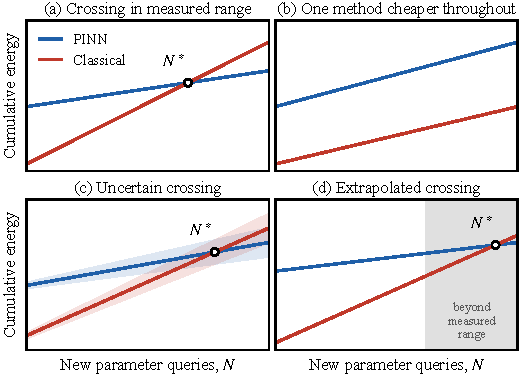
\includegraphics[width=\columnwidth]{breakeven-outcomes.pdf}
\caption{The four outcome classes. The curves are sketches, not data. Bands in (c) show uncertainty. The gray area in (d) lies beyond the largest measured query count.}
\label{fig:outcomes}
\end{figure}

\subsection{Research Questions}
The study asks four questions. None has an assumed answer. (Q1) Does an energy crossover exist within a practical query count? (Q2) Do the energy and runtime crossovers fall at the same $N$? (Q3) How does $\Nstar$ move when the target tightens from $10^{-2}$ to $10^{-3}$? (Q4) Does a crossover claim survive the spread across training seeds?

% ===========================================================================
\section{Solver Design}\label{sec:solvers}

\subsection{Classical Solver}
The classical solver uses five-point finite differences on a uniform grid. The conductivity is taken at cell faces. For the candidate~\eqref{eq:k}, with $k$ read at face midpoints, the matrix is affine in the parameters:
\begin{equation}
A(\boldsymbol{\mu})=A_0+\mu_1A_1+\mu_2A_2 .
\label{eq:affine}
\end{equation}
The three matrices are built once, from the conductivities $1$, $x$, and $y$. Each query forms $A(\boldsymbol{\mu}^\ast)$ with two scaled sparse additions, solves, and maps the result to $G$. The matrix changes with $\boldsymbol{\mu}$, so a factorization cannot be reused across queries. The pilot compares a sparse direct solve with preconditioned conjugate gradient and keeps the faster one. For each target, the solver uses the coarsest grid that passes. CG iteration counts may change with $\boldsymbol{\mu}$, so the per-query cost is recorded for every unseen parameter.

\subsection{Parametric PINN}
One network maps $(x,y,\mu_1,\mu_2)$ to the solution. The inputs are scaled to $[-1,1]$ inside the model. The zero boundary value is built into the output~\cite{sukumar2022,sun2020}:
\begin{equation}
\hat u(x,y;\boldsymbol{\mu})=x(1-x)\,y(1-y)\,v(x,y,\mu_1,\mu_2;\mathbf{w}),
\label{eq:hard}
\end{equation}
where $v$ is the raw network output. Training minimizes the mean squared PDE residual at points sampled from $\Omega\times\Theta$. No solution data is used. The candidate settings come from the project's training plan. The network has three or four tanh layers of width 32 or 64. Adam runs first, with resampled points~\cite{wu2023}. L-BFGS then runs on a fixed Sobol point set~\cite{rathore2024}. Training uses 64-bit floats, unless the pilot shows their cost is too high and 32-bit floats pass~\cite{xu2025}. The stop rule is frozen before the main runs, and no run is stopped by judgment. At least three seeds are trained. Every attempt is logged with its stop reason and a label such as passed, missed target, stalled, or diverged. The deployed model is the seed with the lowest validation error, and all seeds trained under the policy are charged.

% ===========================================================================
\section{Measurement Protocol}\label{sec:measure}

\subsection{Energy Boundary}
Energy is read from hardware counters. RAPL covers the CPU package and memory~\cite{henderson2020,khan2018}. The NVIDIA management interface covers the GPU. The boundary is the same for both methods, even when one device is mostly idle. Each component is also reported on its own. No device reading is called whole-machine electricity. Energy is the counter difference over a window, not one power sample. If a counter is missing, a modeled value may be used only with supervisor approval, and it is labeled as an estimate~\cite{lacoste2019}.

\subsection{Trial Blocks}
Each block starts with a warm-up, which is not counted. Following Yang et~al.~\cite{yang2024}, each GPU query block lasts at least 5~s and runs in four trials with random gaps. Samples taken while power is still rising are dropped. Training is measured as one long window. Thread counts, batching, device placement, and query order are fixed. Clocks are fixed where the hardware allows~\cite{yoo2026,mlperfpower2025}. Idle power is recorded once per session. Both methods record their floating-point precision.

\subsection{Estimates and Uncertainty}
The per-query cost $e$ is block energy divided by the number of queries in the block. A bootstrap over seeds and repeated blocks gives a 95\% interval for $\Nstar$. Before any $\Nstar$ is quoted, we check that each method's per-query cost is stable across block positions and sizes. If it is not, the linear model~\eqref{eq:cost} is reported as unsuitable for that range.

\subsection{Study Ledger}
All study electricity is logged in a separate ledger. This includes the pilot, tuning, validation, failures, and repeats. It is reported apart from the deployment model in~\eqref{eq:retry}.

% ===========================================================================
\section{Reporting Plan}\label{sec:report}

No measurements exist yet. For each target, the results will fill Table~\ref{tab:results}. Each value will carry its 95\% interval. Crossover plots will follow the layout of Fig.~\ref{fig:outcomes}, with measured axes.

\begin{table}[t]
\caption{Reporting format for each target (empty until the trials)}
\label{tab:results}
\centering
\footnotesize
\setlength{\tabcolsep}{2.6pt}
\begin{tabular}{@{}llccccc@{}}
\toprule
Target & Method & Gate & $S$ (kJ) & $e$ (J) & $T$ (s) & $t$ (ms) \\
\midrule
$10^{-2}$ & PINN      & -- & -- & -- & -- & -- \\
          & Classical & -- & -- & -- & -- & -- \\
          & \multicolumn{6}{l}{Crossover: $\Nstar_E$ --, $\Nstar_T$ --; class --} \\
\midrule
$10^{-3}$ & PINN      & -- & -- & -- & -- & -- \\
          & Classical & -- & -- & -- & -- & -- \\
          & \multicolumn{6}{l}{Crossover: $\Nstar_E$ --, $\Nstar_T$ --; class --} \\
\bottomrule
\end{tabular}
\end{table}

% ===========================================================================
\section{Threats to Validity}\label{sec:threats}

\emph{Weak baseline.} An under-tuned classical solver can create a false crossover~\cite{mcgreivy2024}. The affine reuse, the pilot's solver choice, and the coarsest passing grid are meant to prevent this.

\emph{Unequal coverage.} A GPU reading and a CPU reading are not the same system total. Reading one boundary for both methods avoids this. An idle GPU then adds energy to the classical runs, so the per-component view also matters.

\emph{Training variance.} Three seeds give a weak estimate of the pass rate $q$. We will report failure counts, not rates. A low $q$ raises $S_P$ and can move a result into the uncertain class.

\emph{Scope.} The results will hold only for this machine, this PDE family, this parameter box, and these targets. Reduced basis methods~\cite{hesthaven2016} and multigrid solvers are strong options that we do not test. Newer PINN optimizers~\cite{wang2025soap} might lower the training cost. Three of our main sources are preprints~\cite{huang2026review,zhang2026,kapoor2025}.

% ===========================================================================
\section{Conclusion}\label{sec:conclusion}

We have set out how to measure whether, and when, a parametric PINN's training energy and time are paid back by cheaper queries. The comparison is against a finite-difference solver at the same accuracy. The design charges failed runs, reads energy inside one boundary, and sorts each result into one of four outcomes with an interval. The next step is the pilot. It will check the energy counters, test both methods on the 1D heat problem, and freeze the protocol.

\section*{Acknowledgment}
An AI assistant helped draft and edit this paper from the project's research notes. The authors are responsible for its content.

\bibliographystyle{IEEEtran}
\bibliography{../shared/references}

\end{document}
